\documentclass[12pt,letterpaper]{exam}
\usepackage[letterpaper,left=0.5in,right=0.5in,top=0.5in,bottom=0.5in]{geometry}
%\usepackage{toc}

% --- Fonts ---
\usepackage[T1]{fontenc}
\usepackage[utf8]{inputenc}
\usepackage{libertine}

% --- Math ---
\usepackage{amssymb}
\usepackage{amsthm}
\usepackage{mathtools}
\usepackage{bbm}

% --- References ---
\usepackage{hyperref}
\usepackage{cleveref}
\usepackage[style=ieee]{biblatex}       % bibliographies
\addbibresource{../../Schoolwork/Drafts/Mini Prospectus/other/Prospectus.bib}

% --- Other Common Packages ---
\usepackage{booktabs}
\usepackage{graphicx}
\graphicspath{{../figures/}}
\usepackage{subcaption}
%\usepackage{multicol}
%\usepackage[shortlabels]{enumitem}
%\usepackage[table]{xcolor}
\usepackage{wrapfig}
%\usepackage{capt-of}
%\usepackage{tikz}
%\usepackage{pgfplots}
%\usetikzlibrary{shapes,arrows,positioning,patterns}
\usepackage{comment}
\usepackage{minted}
\setmintedinline{bgcolor=gray!10,fontsize=\footnotesize}
\setminted[bash]{bgcolor=gray!10,fontsize=\footnotesize}

%\newcommand\chapter{ X }
\renewcommand{\thequestion}{\textbf{\thesection.\arabic{question}}}
\renewcommand{\questionlabel}{\thequestion}

\usepackage{xpatch}	% This hides the multiple label warning from having
\makeatletter		% multiple question sections.
\xpatchcmd{\questions}
  {question@\arabic{question}}
  {question@\arabic{section}@\arabic{question}}
  {}{}
\makeatother

% -------------------------------- Top Matter -------------------------------- %
\newcommand{\class}{PhD Specialty} % This is the name of the course 
\newcommand{\assignmentname}{Examination} % 
\newcommand{\authorname}{Hosley, Brandon} % 
\newcommand{\workdate}{\today} % 
%\printanswers % this includes the solutions sections

% --------------------------------- Document --------------------------------- %
\begin{document}
\pagestyle{plain}
\thispagestyle{empty}
\noindent
 
% ---------------------------------- Header ---------------------------------- %
\noindent
\begin{tabular*}{\textwidth}{l @{\extracolsep{\fill}} r @{\extracolsep{10pt}} l}
	\textbf{\class} & \textbf{\authorname} &\\%Your name here instead, obviously
	\textbf{\assignmentname } & \textbf{\workdate} & \\
\end{tabular*}\\ 
\rule{\textwidth}{2pt}

% ----------------------------------- Body ----------------------------------- %
\tableofcontents
\hspace*{1em}
\hrule


\section{Dr. Yielding's Questions}

While HARL is indeed a subfield of MARL, the distinction between the 
two can often be unclear or inconsistently used in the literature. 
In the broadest sense, 'heterogeneous' may refer to any MARL scenario 
where the agents are not identical. However, using this broad 
definition risks diluting the practical significance of the term.

To provide a more useful distinction, HARL should be invoked when 
the heterogeneity of the agents is fundamental, essential, or definitional 
rather than merely incidental. 
This means the differences among agents are critical to their roles and 
interactions within the system, not just minor variations.

Prior to my literature review, I would have considered HARL to apply 
specifically to cases where agents are distinct from the outset, 
either in their capabilities (For action-space \(\mathcal{A}\), 
\(\mathcal{A}_1 \neq \mathcal{A}_2\)) or their observation spaces
(\(\mathcal{O}_1 \neq \mathcal{O}_2\)). 
This intrinsic heterogeneity is evident in works like \cite{calvo2018} 
(the Irish conference paper mentioned in Dr. Yielding's question)
and implicitly reflected in \cite{berner2019} (OpenAI Five), 
even though they do not explicitly label their methods as HARL.

The most comprehensive source on HARL usage is Zhong et al. \cite{zhong2024}, 
whose work has greatly influenced my understanding. 
They focus on implementing algorithms that encourage the development of 
heterogeneous policies among agents. 
Their framework increases the likelihood of individual agents converging 
on distinct policies, which I term emergent heterogeneity.

In my prospectus, I also mention a suspicion that this approach might not 
entirely prevent agents from converging on policies that are functionally 
similar, thus lacking true diversity. However, this assertion remains an 
ancillary detail as it is not yet substantiated by empirical evidence.

Therefore, I propose distinguishing between intrinsic heterogeneity, where 
agents are fundamentally different before training, and emergent heterogeneity, 
where differences arise as a result of the learning process. 
In the cases where the heterogeneity of the agents falls below a level of 
functional relevance, and appears to be incidental, I argue that they
should not be labeled as HARL. By maintaining these distinctions, 
we can more accurately categorize and understand the applications and 
implications of HARL and MARL.

Below, I apply these distinctions to the cases proposed:

\begin{questions}
	\question
	HAA2C and HADDPG are among the numerous algorithms proposed by 
	Zhong et al.~\cite{zhong2024}. While it seems reasonable that their 
	algorithms could be applied to situations with intrinsic heterogeneity, 
	their implementations and tests are applied to environments with agents 
	that are functionally the same.

	I intend to implement (at least a subset of) their algorithms to the 
	extent that time allows. In doing so, I hope to either corroborate or 
	contradict their results by comparing them to similar algorithms under 
	different conditions. This exploration aims to identify any apparent 
	advantages of these algorithms when applied to the experimental variables 
	proposed for Contribution 1. These experimental variables represent 
	smaller difficulties that we expect to face in Contributions 2 and 3.
	% -------------------------- End Question -------------------------- %

	\question 
	\begin{parts}
		\part
		The scenario described in this part of the question is, perhaps 
		unintuitively, more akin to single-agent than multi-agent reinforcement 
		learning. This becomes clearer when considering a single agent acting 
		as an 'overlord,' where the observation space is a combination of 
		observations from all the individual agents. The actions taken by this 
		overlord are combinations of actions chosen for each agent. 
		Essentially, a single policy processes the combined observation and 
		outputs the combined action.

		\part
		This example is a strong example of MARL, and because the agents
		utilize copies of a singular policy, this example is free from
		any of the types of heterogeneity described in the answer for question
		1.1.

		\part
		The types of problems accurately described by the scenario provided 
		in this part of the question appear to be a subset of MARL problems 
		and a superset of HARL problems.

		Many MARL algorithms allow the member policies to develop distinctly 
		(e.g., \cite{foerster2017, rashid2018, lowe2020}), but they are 
		not optimized to facilitate the development of distinct policies.

		Zhong et al. \cite{zhong2024} formulate their series of HARL 
		algorithms with optimizations intended to facilitate the development 
		of distinct policies. One weakness of this formulation is that there 
		is no guarantee that the multiple policies will not converge to a 
		behaviorally indistinct set, similar to the concept of 
		carcinization observed in evolutionary biology.

		Thus, the resulting heterogeneity of the agents in these scenarios 
		is not intrinsic but emergent. Whether the algorithm itself is 
		labeled as MARL or HARL is distinguished by intent.
	\end{parts}
	% -------------------------- End Question -------------------------- %

	\question
	Referencing Centralized Training Decentralized Execution (CTDE) 
	and Decentralized Training Decentralized Execution (DTDE) as employed 
	by Li et al. in their FA2A paper \cite{li2023d}, we see that CTDE is 
	the most common format for Actor-Critic based MARL algorithms 
	\cite{foerster2017, rashid2018, lowe2020, li2023d, zhou2023}.

	Li et al. \cite{li2023d} and Wen et al. \cite{wen2021} are the only 
	papers I found that discuss the contrary implementation, DTDE. 
	In both cases, the authors motivate DTDE with practical concerns, 
	particularly the limitations of inter-agent communication in 
	distributed systems. These considerations are important, but the 
	relation to HARL remains the same as described in answer 1.2 (c).
	% -------------------------- End Question -------------------------- %
\end{questions}


\section{Dr. Robbins' Questions}

\begin{wraptable}{R}{0.45\linewidth}
	\centering
	\vspace*{-1em}
	\begin{tabular}{ll}
		Setting & Value \\
		\midrule
		Template & vscode-server \\
		Image & reg.git.act3-ace.com/ace/ \\
			& hub/vscode-server:v0 \\
		Max CPUs & 64\\
		Req. CPUs & 16 \\
		Memory & 64 GB \\
		GPU & None \\
		\bottomrule
	\end{tabular}
	\caption{Container Settings}
	\label{tab:vm_specs}
	\vspace*{-1em}
\end{wraptable}

In addition to being included in the appendices of this exam,
all code used to run the experiments is available on my github at 
\href{https://github.com/bhosley/Specialty-Exam}{
	https://github.com/bhosley/Specialty-Exam}.
It is written to be run on any ANT-Center VSCode server containers,
but should work in a generic virtual environment.
The specifications for the virtual machines used for this experiment
are enumerated in \cref{tab:vm_specs}.

I recommended increasing the ratio of memory to CPU allocation 
for future experiments as the container was substantially closer
to maximum utilization of memory than processing for the duration
of the experiments run for this exam.

The github readme has a short guide for setting up the virtual
environment in the ANT-Center for easy replication.
The answers for this section are drawn from the experiment running script,
also provided in \cref{app:dqn_exp} of this document.

\begin{questions}
\setcounter{question}{0}
	\question
	The Deep Q-network (DQN) implementation \cite{mnih2013,mnih2015}
	implemented in the RLlib framework \cite{liaw2018tune} was used for 
	each of the answers in this section.
	The default results output is readable by tensorboard, 
	but I chose to use the wandb (Weights and Balances) api as well.
	
	To perform this baseline experiment we can call the default script
	(\cref{app:dqn_exp}). We can accomplish a 5 replication test by setting
	\mintinline{bash}|--num-env-runners=5|, however, this overrides the 
	default of 10, so we have chosen not to use it and to keep the default.
	We use the 
	\mint{bash}|python dqn_exp.py --sweep --num-samples=30 --num-env-runners=60|

	\subsubsection*{Round 1 - Bad Results:}
	In the first round of Parameter sweeping, a large number of training runs
	failed to converge on reasonable results. This was somewhat surprising,
	and when examining the parameters there was no immediately obvious pattern.
	Adding the average number of steps per episode to the Comparison 
	(\cref{fig:baseline_1}) shows consistently shorter episodes for poor
	performance.
	\begin{figure}
		\centering
		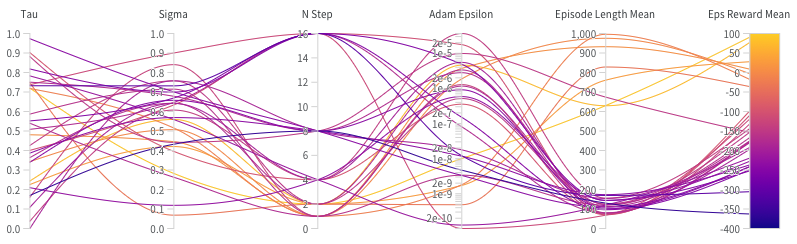
\includegraphics[width=.75\linewidth]{baseline_1.png}
		\caption{Lunar Lander Baseline Experiment 1 Hyperparameters}
		\label{fig:baseline_1}
	\end{figure}
	Further investigation showed that the observation space assigned to the 
	environment from the RLlib registered lunar lander environment was
	significantly different from the correct space.
	Further, manually registering the environment after importing
	it directly from the Farama maintained packages using Ray's environment
	registration function resulted in an outdated observation space,
	less prone to resulting in error, but still problematic.

	Thus we gain two actionable insights. First, we adjust this experiment 
	to use the custom Lunar Lander environment described in the next section, 
	but set to one agent. Second, we identify an update that can be performed 
	by a pull request to the maintainers of RLlib, a contribution to the 
	open-source software I would like to attempt after the submission of this
	exam.



%%%%%%%%%%%%%%%%%%%%%%%%%%%%%%%%%%%%%%%%%%%%%%%%%%%%%%%%%%%%%%%%%%%%%%%%%%%%%%%%
% --------------------------------- Edit Bar --------------------------------- %
%%%%%%%%%%%%%%%%%%%%%%%%%%%%%%%%%%%%%%%%%%%%%%%%%%%%%%%%%%%%%%%%%%%%%%%%%%%%%%%%


	\subsubsection*{Round 2 - Baseline Parameter Sweep:}
	
	%\begin{figure}
	%	\centering
	%	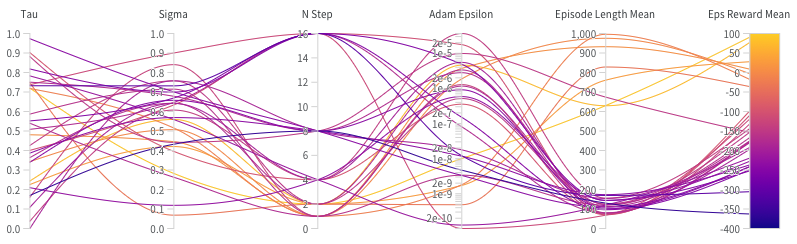
\includegraphics[width=.75\linewidth]{baseline_1.png}
	%	\caption{Lunar Lander Baseline Experiment 1 Hyperparameters}
	%	\label{fig:baseline_1}
	%\end{figure}

	%
	%	Generate appropriate tables and figures to describe the results of your effort.
	%

\end{questions}

\subsection*{Multi-Agent Lunar Lander}
\label{sec:ma-lander}
\addcontentsline{toc}{subsection}{\nameref{sec:ma-lander}}

To modify the Lunar Lander environment to support multiple 
agents it appeared to be possible to simply duplicate all of the
sections that referenced the lander in the original code.
However, to achieve cleaner code, and behavior more consistent with 
Farama's PettingZoo environments, I elected to rewrite the environment
to be more consistent with object oriented programming principles.

\begin{figure}[h]
	\begin{subfigure}{.48\textwidth}
		\centering
		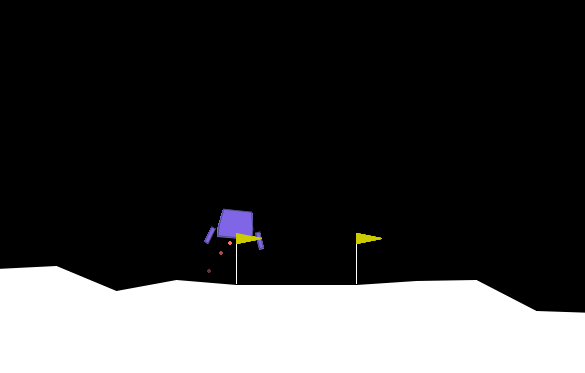
\includegraphics[width=.75\linewidth]{single_lander.png}
		\caption{Original}
		\label{fig:original}
	\end{subfigure}
	\begin{subfigure}{.48\textwidth}
		\centering
		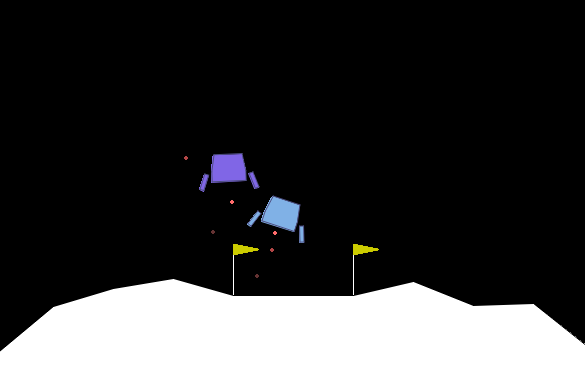
\includegraphics[width=.75\linewidth]{dual_lander.png}
		\caption{With 2 Landers}
	\end{subfigure}
	\\
	\begin{subfigure}{.48\textwidth}
		\centering
		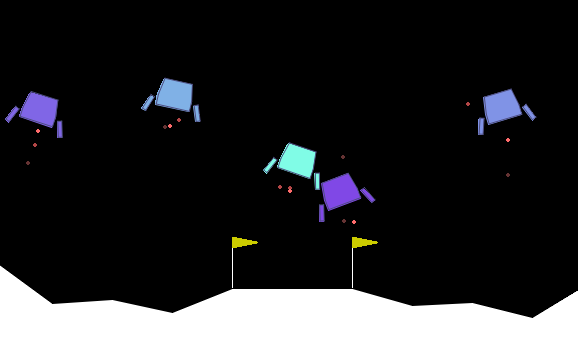
\includegraphics[width=.75\linewidth]{penta_lander_1.png}
		\caption{With 5 Landers}
	\end{subfigure}
	\begin{subfigure}{.48\textwidth}
		\centering
		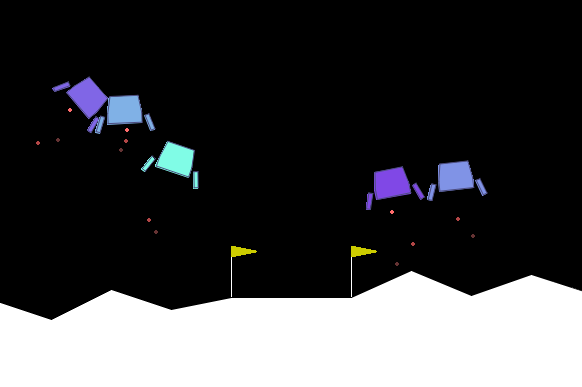
\includegraphics[width=.75\linewidth]{penta_lander_2.png}
		\caption{5 Landers with Collision}
	\end{subfigure}
	\caption{Multi-Agent Lunar Lander}
	\label{fig:landers}
\end{figure}

This trivialized the retention of the environmental physics,
and made it very easy for the new environment to comply with both the 
AEC (Agent Environment Cycle; or sequential) and parallel execution 
methods used in the PettingZoo API. Further, this made it much easier 
to retain the heuristic solution from the original environment.
\Cref{fig:landers} shows several screen shots from the resulting environment
when rendered. 

While an AEC version of this custom environment was constructed,
it was not used for this exam. AEC iterates through the list of agents, 
allowing the agent to select an action and steps the environment with that 
action before moving to the next agent, in a manner similar to a board game.
Such an implement doesn't necessarily contribute value to the 
multi agent Lunar Lander sim, and in fact, causes problems if the physics
of the environment are not adjusted as the number of landers is increased.
Using the heuristic as a measure, the AEC environment becomes unsolvable
with 3 or more landers. The effect of their actions must be scaled to overcome
the wait time between their turns, otherwise they simple crash, unable to 
overcome gravity.

The parallel version of the environment was used for this exam, and required 
only one major assumption, centering around collisions between the landers. 
Lunar Lander uses the Box2D package to model the moon surface and lander.
The most expedient method to address collisions using Box2D was to detect
only contact with the lander's body.
If any other object touches a lander's body it is considered a crash.
As written, the Box2D contact detection does not distinguish between 
what the secondary object is, if the legs of the lander where
included, contact with lunar surface would show as a crash.
Thus I chose not to include the legs contact detection for collisions.
The effective result is that if two lander's legs touch it is not treated
as a crash, however, if one lander's legs touch another's body module
it is treated as a crash and thus a failure.

\begin{questions}
\setcounter{question}{1}
	\question \textbf{Formulate a Markov Game:}
	The Markov game that represents the multi-agent version of this
	environment is an extension of the Markov Decision Process (MDP)
	that represents the original Lunar Lander environment.
	The formulation presented here will be used to describe the 
	interactions in all of the questions that follow.

	\emph{Agent:} The agent is represented as a member of set of agents 
	\(n\in N\).

	\emph{State Space:} Let \(\mathcal{S}\) be the state space. 
	Then, \(\mathcal{S} \equiv s^N\), where 
	\[s = \begin{cases}
		x \in [-2.5,2.5]   & \text{Position of } n \text{ in } x \\
		y \in [-2.5,2.5]   & \text{Position of } n \text{ in } y \\
		\vec{x} \in [-10,10] & \text{Velocity of } n \text{ in } x \\
		\vec{y} \in [-10,10] & \text{Velocity of } n \text{ in } y \\
		\omega \in [-2\pi,2\pi] & \text{Angle of } n\\
		\vec{\omega} \in [-10,10] & \text{Angular Velocity of } n\\
		\mathbb{I}(\text{leg 1}) \in\{0,1\}  & \text{Leg on ground}\\
		\mathbb{I}(\text{leg 2}) \in\{0,1\}  & \text{Leg on ground}
	\end{cases}\]

	\emph{Action Space:} Let \(\mathcal{A}\) be the action space.
	Then, \(\mathcal{A} \equiv a^N\), where 
	\[a \in \begin{cases}
		0 & \text{No-Op} \\
		1 & \text{Fire Left Engine} \\
		2 & \text{Fire Main Engine} \\
		3 & \text{Fire Right Engine}
	\end{cases}\]

	\emph{Transition Probability:} The transition probability for
	each agent \(n\) remains the same as the original environment,
	\[P_n(s_{n,t+1}|s_{n,t},a_{n,t}) \cong \begin{cases}
		\text{Dispersion} \sim U(-1,1) \\
		\text{Wind(Linear)} = \tanh(\sin(2 k x) + \sin(\pi k x)) \\
		\text{Wind(Rotate)} = \tanh(\sin(2 k x) + \sin(\pi k x)) \\
	\end{cases}\]
	Thus the transition probability for the game as a whole is
	\[P(s_{t+1}|s_{t},a_{t}) = \prod_{n\in N} P_n\]

	\emph{Reward:} The reward structure is similarly retained from 
	the original Lunar Lander environment. Specifically, the reward
	at time \(t\) is defined as
	\(r(t) = \sum_{n\in N} r_n(t)\)
	where
	\begin{align*}
        r_n(t) = \\
        & \pm 100                   & \text{End-state, crash or land} \\
        & +10 (s_{t,6} + s_{t,7})   & \text{leg(s) on ground} \\
        & -a_n(t)\cdot [0,0.03,0.3,0.03] & \text{thruster cost} \\
        & - 100\sqrt{s_{n}(t)_0^2+s_{n}(t)_1^2} & \text{Distance} \\
        & - 100\sqrt{s_{n}(t)_2^2+s_{n}(t)_3^2} & \text{Velocity} \\
        & - 100|\omega_n(t)| & \text{Tilt}
    \end{align*}

	\question \textbf{DQN Single-Agent Controller:}
	This problem was approached using a wrapper class around the
	custom multi-agent environment to translate the between the 
	multi-agent environment and single-agent policy. 
	The proxy single-agent state/observation was formed by simply 
	concatenating the state vectors of each agent.

	The modified action space for this problem is
	\(\mathcal{B} \equiv \mathcal{A}^N\).
	To relate the two action spaces for this problem I use the function,
	\[ b = \sum_{}^{} a_n \times \dim(a)^n. \]
	Then to translate the modified action into the agent-action vector 
	necessary for the multi-agent environment I use the following function,
	\[ \mathbf{a} = \{b/\dim(a)^n \mod\dim(a) \}_{n\in N} \] which 
	relies on \(\dim(\mathcal{A}_n)=\dim(\mathcal{A}_m)\forall\ n,m\in N\),
	an assumption that I note as it is true for this problem, 
	limits some generality.
	The policy can thus be represented as \(\pi(b \big| [s_n]_{n\in N})\).

	Finally, the experiment can be replicated using the command:	
\mint{bash}|python dqn_exp.py --SA --sweep --num-samples=30 --num-env-runners=30|
	

	%
	%	Generate appropriate tables and figures to describe the results of your effort.
	%


	\question \textbf{NoPS - No Parameter Sharing:}
	This experiment uses a distinct policy for each agent, 
	\(\pi_n(a_n|s_n)\),
	and can be replicated using:
\mint{bash}|python src/dqn_exp.py --NoPS --sweep --num-samples=30 --num-env-runners=30|
	

	%
	%	Generate appropriate tables and figures to describe the results of your effort.
	%
	
	\question \textbf{FuPS - Full Parameter Sharing:}
	This experiment uses a shared policy for each agent, 
	\(\pi(a_n|s_n)\),
	and can be replicated using:
\mint{bash}|python src/dqn_exp.py --FuPS --sweep --num-samples=30 --num-env-runners=30|

	%
	%	Generate appropriate tables and figures to describe the results of your effort.
	%

	\question \textbf{Results Comparisons:}
\end{questions}

	%
	%	Generate appropriate tables and figures to describe the results of your effort.
	%


\section{Dr. Cox's Questions}
%\begin{questions}
%	\question
%	\question
%\end{questions}

\begin{comment}
Problem 1:


Contribution 1 seems very broadly scoped, and somewhat ill defined (especially when compared
to the well-defined and scoped contribution 2). Please add, at least the following, explicit details
to contribution 1 in terms of:
a. Which cooperative tasks will be explored?
b. Which competitive tasks will be explored?
c. Which algorithms will be explored?
d. Which environments will be explored?
e. Which league frameworks will be explored?
Overall, I am looking for a significant expansion of the methodology of contribution 1 similar to
what we would expect from the final manuscript. Since Contribution 1’s timeline overlaps
significantly with June and July it is reasonable that such details should exist or can be developed.
My concern is that contribution 1 may need to be rescoped to a narrower focus, or split into
multiple papers each with a tighter focus.



Problem 2:


Execute a very small practical experiment of contribution 1: For example, choose 1 MARL
algorithm and 1 HARL algorithm, choose 1 environment with a cooperative task. Write up a minipaper on this experiment. You should have an introduction that motivates the problem, a brief
literature review, a detailed methodology section along with a summary of results. The goal of
this question is to test your ability to implement a very small scale experiment aligned with your
proposed contribution 1.




\end{comment}




\clearpage
\appendix

\section{Experiment Running Script}
\label{app:dqn_exp}
\inputminted[
	fontsize=\footnotesize,
	%bgcolor=gray!05,
	linenos
	]{python3}{../src/dqn_exp.py}

\clearpage
\section{Multi-Agent Lunar Lander}
\label{app:ma-lander}
\inputminted[fontsize=\footnotesize, linenos]{python}{../src/multi_lander.py}

\end{document}
